\documentclass[twoside,11pt,a4paper]{article}
 
\usepackage[utf8]{inputenc}
\usepackage{amsmath, amssymb, latexsym}
\usepackage{sidecap}
 
\usepackage{tikz}
\usetikzlibrary{decorations.pathreplacing}
\usepackage[colorinlistoftodos, color=green!40, prependcaption]{todonotes}
\usepackage{booktabs}
\usepackage{comment}
\usetikzlibrary{positioning,chains}
\usepackage{tikz}
\usepackage{lipsum,adjustbox}
\usepackage{empheq} 
\usetikzlibrary{shapes,arrows,positioning}
\usetikzlibrary{fit, arrows.meta, shapes}
\usetikzlibrary{external}
\tikzexternalize % activate!
\newcommand{\subsubsubsection}[1]{\paragraph{#1}\mbox{}\\}
\setcounter{secnumdepth}{4}
\setcounter{tocdepth}{4}

\mathtoolsset{showonlyrefs=false} 
\usepackage{xcolor}
\usepackage{hyperref} % For hyperlinks in the PDF
%\setlength{\marginparwidth}{2.5cm}
\bibliographystyle{apsrev4-1}
%\bibliographystyle{apalike}
\usepackage{tikz}
\usetikzlibrary{quantikz}
% defines the color of hyperref objects
% Blending two colors:  blue!80!black  =  .8 blue and 0.2 black       % automagic cross-referencing
\hypersetup{ % this is just my personal choice, feel free to change things
    colorlinks,
    linkcolor={red!50!black},
    citecolor={blue!50!black},
    urlcolor={blue!80!black}}

\usepackage{listings}
\lstset{language=C, keywordstyle={\bfseries \color{blue}}}

\bibliographystyle{apsrev4-1}




\begin{document}
 \begin{figure}
    \begin{adjustbox}{width=0.8\textwidth}
    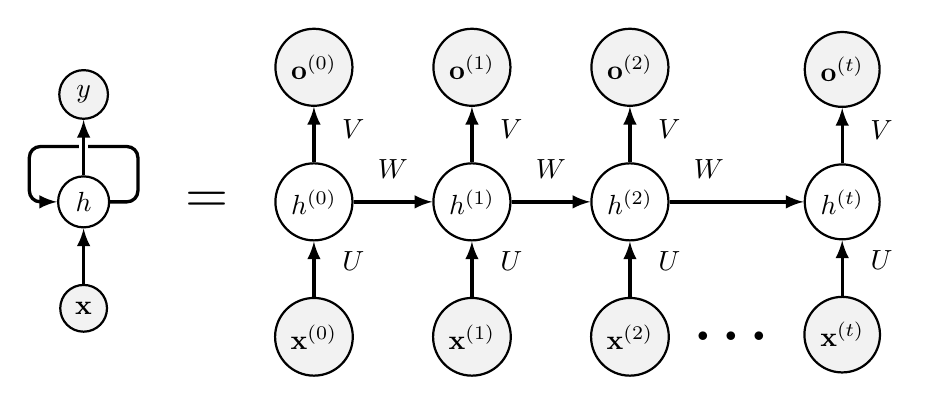
\begin{tikzpicture}[item/.style={circle,draw,thick,align=center},
itemc/.style={item,on chain,join}]
 \begin{scope}[start chain=going right,nodes=itemc,every
 join/.style={-latex,very thick},local bounding box=chain]
 \path node (A0) {$h^{(0)}$} node (A1) {$h^{(1)}$} node (A2) {$h^{(2)}$} node[xshift=2em] (At)
 {$h^{(t)}$};
 \end{scope}
 \node[left=1em of chain,scale=2] (eq) {$=$};
 \node[left=2em of eq,item] (AL) {$h$};
 \path (AL.west) ++ (-1em,2em) coordinate (aux);
 \draw[very thick,-latex,rounded corners] (AL.east) -| ++ (1em,2em) -- (aux) 
 |- (AL.west);
 \foreach \X in {0,1,2,t} 
     {\draw[very thick,-latex] (A\X.north) -- ++ (0,2em)
     node[above,item,fill=gray!10] (h\X) {$\mathbf{o}^{(\X)}$};
     %\ifthenelse{\X!=t;}{ \path (A\X.east) -- ++ (1,1em) node[midway, above] {$W$};};
     \draw[very thick,latex-] (A\X.south) -- ++ (0,-2em)
     node[below,item,fill=gray!10] (x\X) {$\mathbf{x}^{(\X)}$};}
 \draw[white,line width=0.8ex] (AL.north) -- ++ (0,1.9em);
 \draw[very thick,-latex] (AL.north) -- ++ (0,2em)
 node[above,item,fill=gray!10] {$y$};

 \draw[very thick,latex-] (AL.south) -- ++ (0,-2em)
 node[below,item,fill=gray!10] {$\mathbf{x}$};
 \path (x2) -- (xt) node[midway,scale=2,font=\bfseries] {\dots};

\foreach \X in {0,1,2} 
    \path (A\X.east) -- ++ (1,1em) node[midway, above] {$W$};
\foreach \X in {0,1,2, t} 
    \path (A\X.north) -- ++ (1,1em) node[midway, above] {$V$};
\foreach \X in {0,1,2,t} 
    \path (A\X.south) -- ++ (1,0em) node[midway, below] {$U$};
\end{tikzpicture}
\end{adjustbox}
\end{figure}
\end{center}


\end{document}


